A continuación se muestra la representación del árbol de versiones del proyecto, con los siguientes elementos:
\begin{itemize}
    \item \textbf{Branch/Rama}: En naranja, muestra el punto final de cada rama.
    \item \textbf{Commit}: En azul, muestra los distintos objetos listados en el apartado anterior.
    \item \textbf{Head/Cabeza}: En rosa, muestra el punto en el que actualmente se encuentra el proyecto.
\end{itemize}
Es necesario puntualizar que los distintos elementos están unidos por flechas. Estas flechas indican dependencia hacia el elemento inmediatamente anterior en la historia.
\begin{multicols}{2}
    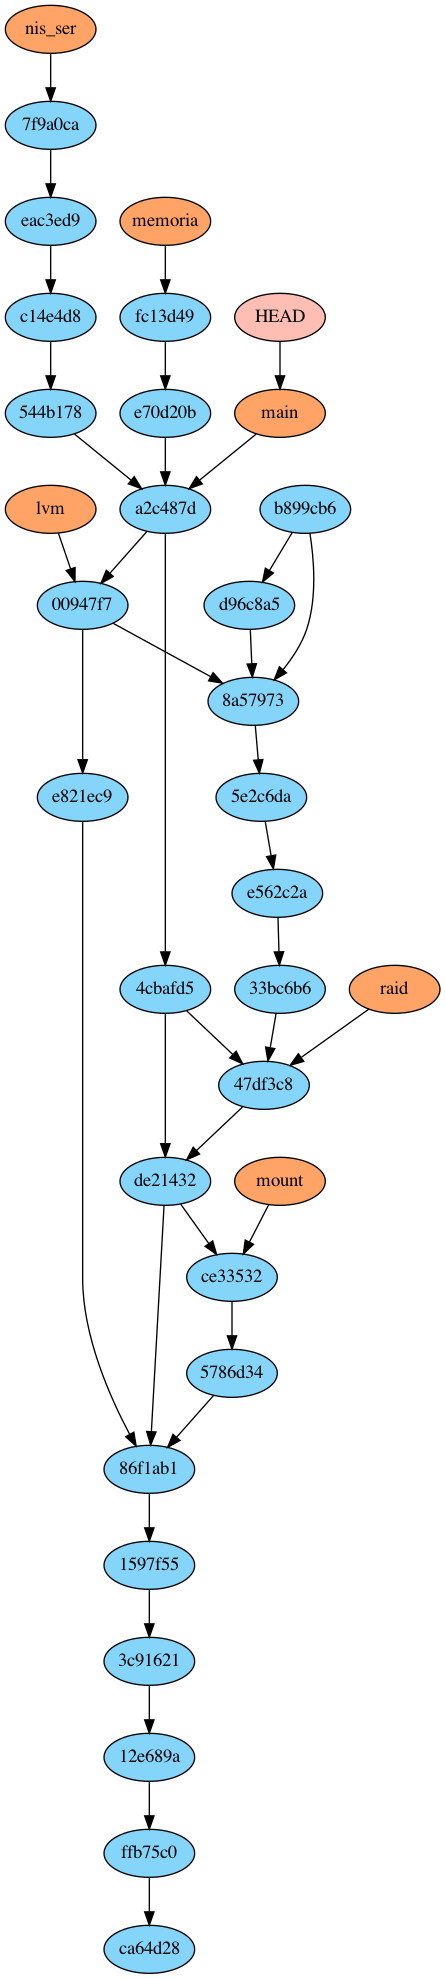
\includegraphics[trim={0 30cm 0 0}, clip, width=0.4\textwidth]{includes/graph.png}

    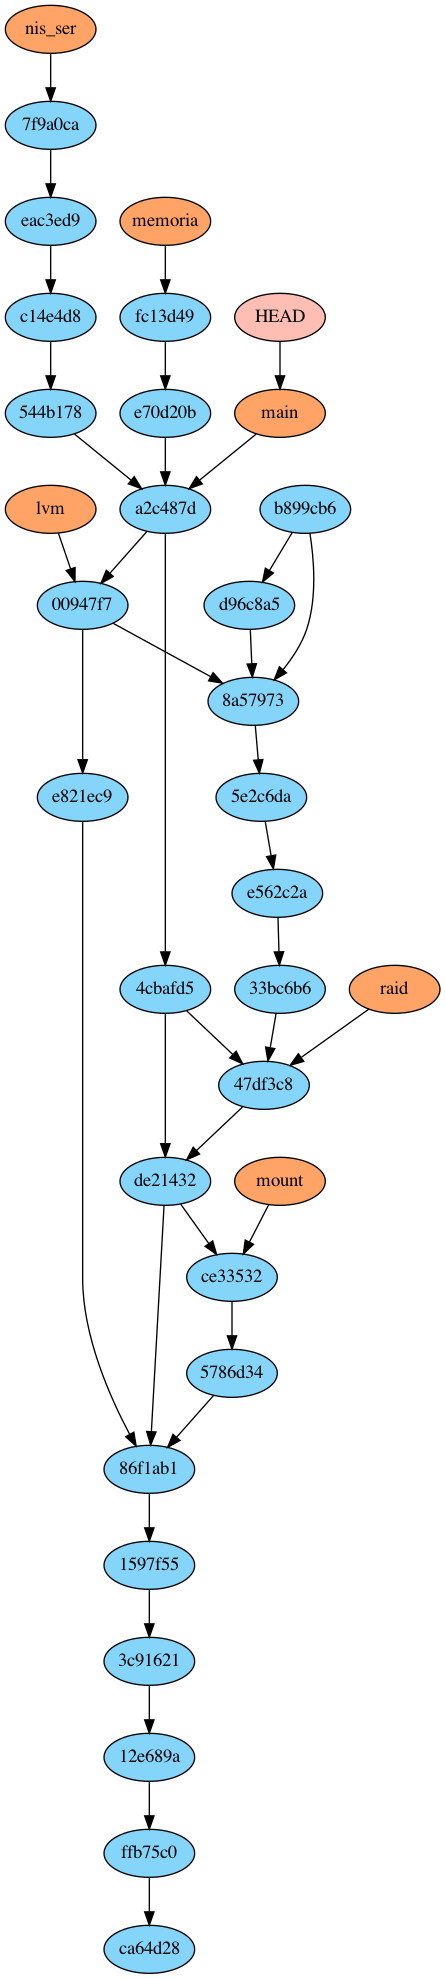
\includegraphics[trim={0 0 0 30cm}, clip, width=0.4\textwidth]{includes/graph.png}
\end{multicols}